\documentclass[conference]{sig-alternate-05-2015}
\usepackage{graphicx}
\usepackage{epstopdf}
\usepackage{epsfig}
\usepackage{color}
\usepackage{pseudocode}
\usepackage{listings}
\usepackage{etoolbox}
\usepackage[table]{xcolor}
\usepackage{tabularx}
\usepackage{booktabs}
\usepackage{enumitem}
\usepackage{amsfonts}
\usepackage[boxruled]{algorithm2e}
\usepackage{ragged2e}
\usepackage{mathtools}
\usepackage{stmaryrd}
\usepackage{amsmath}
\usepackage{pifont}
\usepackage{multirow}
\usepackage{xcolor}
\usepackage{xspace} %for leaving a space after a string macro, see http below
\usepackage{cite}
\usepackage{amssymb}
\usepackage[bookmarks=false]{hyperref}
\usepackage[font=bf]{caption}
\usepackage{fp}
\usepackage{subcaption}
\usepackage{siunitx}
\usepackage{listings}
\lstset{
    frame=single,
    breaklines=true,
    postbreak=\raisebox{0ex}[0ex][0ex]{\ensuremath{\color{red}\hookrightarrow\space}}
}

% caption setup
\captionsetup[table]{position=below}
\captionsetup[figure]{position=below}

% thousand comma separator
\sisetup{group-separator = {,}}

\newcommand{\note}[1]{\textcolor{blue}{[#1]}}
\newcommand{\jason}[1]{\textcolor{red}{[#1]}}


\makeatletter
\def\@copyrightspace{\relax}
\makeatother

\begin{document}
\title{An Improved Approach to breaking Audio CAPTCHAs using Noise Removal and Deep Learning}
\numberofauthors{2}
\author{
\alignauthor Varshini Sampath\\
\affaddr{University of Illinois at Chicago}\\
\affaddr{Chicago, IL, USA}\\
\affaddr{vsampa3@uic.edu}
%\affaddr{Computer Science Dept.}\\
%
\alignauthor Iasonas Polakis\\
\affaddr{University of Illinois at Chicago}\\
\affaddr{Chicago, IL, USA}\\
\affaddr{polakis@uic.edu}
}

\maketitle

\section{Abstract}\mbox{}\
\label{sec:abstract}

CAPTCHA is a backronym for Completely Automated Public Turing test to tell Computers and Humans Apart. As the name suggests, they are automated tests designed to control access to computer systems by distinguishing humans from bots. Since their launch in 2000, websites have used them extensively to prevent bot account creation and spam. There are many types of tests devised for CAPTCHAS in the past. The most common CAPTCHAS are text based, where an image is shown to the users which contains distorted text. Users are asked to read and recognize this text and type the text they see into a textbox that is situated next to the image. Some other common types of CAPTCHAs include tasks of selecting a single or multiple similar images among many heterogeneous images, solving math puzzles, recognizing 3D text, clicking or dragging moving elements, locating text or numbers in a video, etc. \newline

For a long time now, researchers have tested the strength of text CAPTCHAs and using the latest advancements in computer vision, have been able to break text CAPTCHAs with an accuracy of up to 77\% \cite{ebay:machine-noise}. The version 2 ReCAPTCHA by Google employs checkbox and image CAPTCHAs which again, after scrutiny, have been rendered broken with an accuracy of 70.78\% \cite{recurrent:machine-noise}. Ever since CAPTCHAs have been introduced, companies have built their own CAPTCHA systems and have used them to prevent bot activity on their web pages. Also, a number of enterprise solutions that offer CAPTCHA systems as a service have since emerged. Although CAPTCHAs have become very common, users often encounter CAPTCHAs which are hard even for humans to solve. As there is very less or no margin for error to prevent bot activity, users often end up making multiple attempts to solve a challenge. It has been shown that CAPTCHA challenges frustrate users and it negatively impacts the experience and traffic of a website \cite{distil}.\newline

Commercial CAPTCHA services can be utilized by users by signing up with one of the CAPTCHA providers and including a few lines of their code on the target web pages. ReCAPTCHA is one such service offered by Google. Text and image challenges are the most common CAPTCHAs offered by these services which are implemented on web pages to prevent bots from filling web forms automatically. But a drawback with these CAPTCHA systems is that certain groups of people, especially the visually impaired, find it difficult to use them. Thus, audio challenges were introduced specifically to help computer systems be accessible to the visually impaired. The caveat with this approach is that these audio CAPTCHAs open a new ground for exploitation for attackers.\newline

While there has been a lot of prior work done on breaking text and image CAPTCHAs, audio CAPTCHAs have not been studied to such great detail. In this work, we present a survey of all the audio CAPTCHA services that are currently used and show how we used our system to automate the solving of these challenges using existing, off-the-shelf speech recognition services. We found that the latest version of ReCAPTCHA is very vulnerable to our attack.\newline

  



\section{Introduction}
\label{sec:intro}

\note{First paragraph sets the context.}
While automated attacks continue to plague the Internet, the number
of users from around the world going online has reached unprecedented levels.
Thus, it is crucial to deploy user-friendly mechanisms for preventing bots without
becoming obstacles to legitimate users.

\note{Second paragraph is more specific. Talk about audio captchas, give some relevant statistics.}

According to the World Health Organization 285 million people have some form of visual impairment~\cite{impaired}.

Captchas present an interesting dilemma from a design standpoint, as they are an exemplary instance 
of usability and security being at direct contradiction. Adding more noise (or distortion) to combat 
automated solvers will also have a significant negative effect on the ability of users to actually
solve challenges.

Previous work has found that popular audio captchas are more difficult than their visual counterparts,
which was also corroborated by a subsequent systematic evaluation of users' ability to solve various types of
captchas~\cite{captchas-are-hard}.


\note{Third paragraph is about what has been done before, what has changed and what is missing.}

\note{Fourth paragraph talks about what we have done, describes our system.}

In this work, we consider multiple leading CAPTCHA providers which also provide an optional audio 
challenge along with the traditional text or image challenge. To solve these challenges, we consider 
multiple online speech recognition APIs (which we will henceforth refer to as ``solvers'').

\note{Fifth paragraph gives some of our important results.}

Overall, the main contributions of our work are:

\begin{itemize}

\item We present an extensive evaluation of the audio captcha ecosystem, and demonstrate how available services 
can be broken using off-the-shelf speech recognition services.

\item We bla bla bla.

\item We bla bla bla.

\end{itemize}



\section{Previous Work}\mbox{} \
\label{sec:previous}

Although not as extensively studied as the text versions of CAPTCHAs, there have been several studies in the past which have tested and evaluated of audio challenges. The challenge in breaking an audio CAPTCHA lies in automatically recognizing the sequence of spoken words in the audio while ignoring the noise that is added to the file. There is no universally agreed upon value for the success rate to consider a system broken, although the fact that the trade-off between security and usability needs to be taken into account as well. The study by Chellapilla et al. \cite{chellapilla2005designing} suggests that the success rate of a bot must be less than 0.01\%, whereas Bursztein et al. \cite{bursztein2011failure} suggest that the success rate be 1\%, and 5\% by Tam et al. \cite{meutzner2016toward}. \newline

The above numbers depend heavily upon many other factors than just being able to successfully transcribing the audio. This implies that the threat model should not take into account just the transcription, but also factors like rate-limiting and the threat also increases with increase in the number of resources that is at the attacker's disposal. \newline

Recent years have seen an increase in the number of studies in breaking audio challenges. It has been shown that audio challenges very prone to attack with ever increasing advancements in the domain of machine learning. As audio challenges consist of a very limited corpus in the form of digits and alphabets and a narrow form of accents, the defense of audio challenges is very less. Existing studies show that most audio CAPTCHAs can be broken by means of machine learning techniques at relatively low costs \cite{bursztein2011failure,meutzner2016toward,bursztein2009decaptcha}. Hence, additional defenses in the form of IP address geo location, mouse movement, response times, user agents, cookies, etc. are deployed. \newline

Sivakorn et al. \cite{sivakorn2016robot} demonstrate an extremely effective system that solves the state-of-the-art ReCAPTCHA's image based CAPTCHAs with an accuracy of over 70\% and Facebook's image CAPTCHA with an accuracy of over 83\%. This led us to test the accuracy of audio based CAPTCHA systems from different services. We found that the existing mechanisms in place include rate limiting the number of challenges that are served per IP for every device, including background noise to prevent speech recognizers from recognizing the audio CAPTCHAs automatically. We demonstrate that these limits can be bypassed and that the speech recognizers can be tuned to recognize digits, alphabets and words even with background noise.\newline

The success rates for breaking audio CAPTCHAs reported in recent studies are very high. Bursztein et al. \cite{bursztein2011failure} broke the audio challenges of Yahoo, Microsoft, and eBay with a success rate of 45\%, 49\%, and 83\% respectively. Sano et al. \cite{sano2013solving} and Meutzner et al. \cite{meutzner2014using} broke Google's reCAPTCHA with 52\% and 63\% accuracy respectively. There have also been studies that have used state-of-the-art automatic speech recognition techniques, based on hidden Markov models (HMMs).



\section{Breaking Audio CAPTCHAs - Our Approach}
\label{sec:ourapproach}

We did a large-scale study of the security of audio challenges from eight different CAPTCHA providers and websites including Apple, BotDetect, CaptchasNet, Live, Google reCAPTCHA v1, Google reCAPTCHA v2, SecureImage and Telerik. We built web crawlers to scrape the audio challenges from these services, solve them using solvers based on speech recognition services and input back the results in the CAPTCHA textbox. We evaluated our system initially with 50 CAPTCHAs each to identify the best solver and then tested the best solver for each CAPTCHA system with 1000 challenges.\newline

The results of our experiments are given in Fig 2. We found that all of the 8 CAPTCHA systems that we analyzed could be broken with our solvers, despite background noises and the rate limiting that some providers implement. This includes the most popular CAPTCHA system in use - Google's reCAPTCHA (98.3\%) and BotDetect (24.6\%), which is popularly used in government websites. \newline

In this paper, we propose to improve the accuracy of our automated solvers by using audio processing techniques. We identify a sequence of actions like Amplification, Noise Reduction, Low-pass audio filtering, etc that work best for each CAPTCHA system in reducing background noise and making the audio more discernible. For this, we use a free open-source cross-platform audio editor called Audacity. We build Action Chains that describe the set of actions specific to each CAPTCHA system and pass our audio file obtained while solving the CAPTCHAs, real-time, to Audacity. Audacity then cleans up the audio using predefined Action Chains and gives the denoised file back to our system. We observe that the accuracy of our solvers improves significantly for certain CAPTCHA systems like Telerik, Apple and Captchas.net.\newline

Finally, we build an offline neural network based classifier with Intel's Deep Learning system for speech called the \textbf{deepspeech}. We initially build this for SecureImage, identified to have the strongest audio challenges among the eight, based on the very low rate of accuracy from our experiments (3\%). We plan to extend this idea and create classification models for each of the other CAPTCHA systems as a possible future work.\newline

Since SecureImage is an open-source CAPTCHA system, we create a training dataset of 1000 audio sample files mixed with their background noises and train our deepspeech classifier with the truth values. We train our system to create a deep learning model and evaluate the model with a test dataset.\newline

We consider the following to be our main technical contributions in this paper:

\begin{itemize}
\item We present a novel, low-cost approach to breaking audio CAPTCHAs and improving their accuracy by audio processing techniques.
\item We evaluate our improvised system against all eight services by breaking 1000 CAPTCHAs each using the best solver identified after denoising and observe improvement in accuracy. 
\item Our biggest contribution was in proving that audio CAPTCHAs can be solved by open-source services and audio tools that are readily available in the market, with very less effort. This is because speech recognition services developed by big companies like Google, IBM Watson, etc, themselves do a lot of audio processing, noise filtering and machine learning in the background.
\item We are also in the process of creating a neural-network based classifier for speech recognition that can work as an offline audio CAPTCHA solver.
\end{itemize}


\begin{figure}[t]
   \centering
   \includegraphics[width=\columnwidth]{figures/res1.png}.
   \caption{Results from our initial approach, before noise reduction.}
   \label{fig:results1}
\end{figure}


\section{Literature Review}
\label{sec:noisereduction}

This section gives a brief overview of what constitutes noise when it comes to human speech, a classification of the different kinds of noise and the audio processing techniques we used in our system to clean up the audio files.

\subsection{Sound}
Sound is created by alternate compression and decompression of particles of the air. This causes the air pressure to fall and rise in the form of waves. Frequency (pitch) and amplitude (loudness) are the two main characteristics of sound. \textbf{Frequency} is the number of times that the air is compressed and decompressed in a second, and is measured in cycles per second, or Hertz (Hz). Low frequency produces a low pitched, bass sound. High frequency produces a high pitched, whistle-like sound. Human ears respond to frequencies between 20Hz and 20,000Hz. \textbf{Amplitude} is the amount of sound energy reaching the eardrum, and is measured in decibels (dB). The safe range of amplitude for a human ear is 0 to 140dB.\newline

\subsection{Noise in Speech}
The human voice produces frequencies between 500Hz and 2,000Hz. Background noises have higher frequency levels than speech. The comprehension of speech is affected by both amplitude of the background noise and the amplitude of the voice itself. The average amplitude of a human voice in a room at a distance of one meter lies within the following ranges:
\begin{itemize}
\item Conversation	60-65dB
\item Dictation	65-70dB
\item Calling out	80-85dB 
\end{itemize}
The general background noise level must be at least 10dB lesser than these levels if the sound of the voice is to be heard clearly.\newline

\subsection{Classification of noise}
Noise can be broadly classified into 2 kinds - Internal noise and External noise.\newline

\textbf{Internal noise} is noise generated within the receiver or communication system. Colour noises like white noise, pink noise, brown noise,etc are examples of internal noises with specific characteristics, that can sometimes be manually added to mask other disrupting background noises. \textbf{External noise} is noise generated external to the system. So, all kinds of background noise come under this category.\newline

\subsection{Audacity}
We looked for a free, open-source, light-weight digital audio editing tool that was available in the market because our goal was to build a low-cost Audio CAPTCHA breaker. For this reason, we selected Audacity. Audacity is a free digital audio editor and recording tool that is available for Unix, Linux, OSX and Windows platforms. It has a number of built-in audio processing mechanisms that can be fine-tuned to our needs.\newline

\subsection{Audio processing techniques}
There are several audio processing techniques that are commonly used to remove noise and make recordings clearer in audio post-processing. All these techniques are available a single-click away in Audacity. So we exploit these functionalities without having to worry about the algorithm and the implementation. The following are some of the audio processing techniques that we use in this paper.\newline

\begin{itemize}
\item \textbf{Amplification} : Amplification is the process of increasing the amplitude of the audio by a certain amount or ratio. It just makes the audio sounding louder.
\item \textbf{Equalization} : Equalization is the process of adjusting the frequency response in an audio after recording. It is generally used to make certain sounds in an audio more prominent than others. We specifically use it to make vocal sounds louder and the background noises quieter.
\item \textbf{Normalization}: Normalization is done to set the peak amplitude of a track. A normalizer identifies the peak amplitude in the track and the maximum allowed amplitude and calculates gain as the difference between these two values. It then applies this gain for the entire track.
\item \textbf{Noise Gate} : Noise gates are used to remove constant background noises like hiss sounds, murmurs, leaf rustles, etc. It does this by allowing signals above a threshold amplitude value to pass through the gate, while blocking everything below.
\item \textbf{Noise Filter} : A noise filter is used to remove frequencies that do not fall within a certain range. To accomplish this, it uses 2 filters - a low pass filter that attenuates frequencies lower than  particular value and a high pass filter that attenuates frequencies higher than a particular value.
\item \textbf{Noise Reduction} : This technique samples a piece of the audio as a noise profile and applies a reduction in amplitude to the parts of the audio that has this noise.
\end{itemize}



\begin{figure}[t]
   \centering
   \includegraphics[width=\columnwidth]{figures/Picture1.png}.
   \caption{The ReCAPTCHA widget: Users can play the audio, download the file or request for a new challenge.}
   \label{fig:recaptcha}
\end{figure}

\section{System Overview}
\label{sec:design}

\subsection{Generic System}\mbox{} \
\label{sec:generic}

Our system consists of a crawler that loads the required page, finds the audio element in the page and downloads it. It then converts the audio file into the required audio format and hands it over to another system that connects to the speech recognition web services. Once the transcript is obtained from the service, it hands over the result to the first system that fills the CAPTCHA response and submits the form/challenge.\newline

To build the crawler, we used a Python script with Selenium and ChromeDriver. The script recursively loads the URL that has been hard coded into the system and with Selenium, we fire up the ChromeDriver. Selenium helps in finding the required elements on the page and manipulate them. Once it finds the audio element on the page, it is downloaded and if the file is in MP3 format, we use the Pydub library to convert the file to WAV/FLAC format. We did this as IBM Watson's Speech to Text API expects only a WAV file and Google Speech API expects a FLAC file. These two files are stored with the timestamp of when the first file was initially downloaded.\newline

Next, the control is transferred to the solver script. We implemented this in Node.JS and we used the Naked library available for Python to execute a JavaScript file. The Node.JS script is fired up that takes the converted file and sends it to the appropriate solver using its API and gets back the response. In the case when the solver gives a list of alternative transcriptions for each recognized sound, we select the most appropriate one among them.\newline

We did not require transferring control to the Node.JS module for the Google solvers as we used the Python implementations of Google Speech API.To achieve this, we used the Google Speech API Client module that is available to install via the "pip" command for Python and setting up the credentials via a JSON file that can be downloaded by registering for a new application with the Google Cloud platform. \newline

The script then builds the response based on this and sends it back to the Python script. It then enters the response into the response box using Selenium, and the challenge is submitted. Once it is submitted, we look for some element on the page that is generated which tells the user if the submitted response was correct or not. We again crawl the page for this element and gather this result. We next store these results in a CSV file along with the file name for each challenge we solve. \newline

\subsection{Tweaking for ReCAPTCHA}
\label{sec:recaptcha}

We found that ReCAPTCHA had implemented rate limitation (we talk about this in detail in the forthcoming section). To overcome this limitation, we had to tweak our script to generate random user agent strings that would allow us to bypass the limit. It also generated the audio in MP3 format that had to be converted into WAV. \newline

\subsection{Tweaking for Captchas.net and Telerik}
\label{sec:captchasnet}

Captchas.net and Telerik CAPTCHAs spell out NATO characters and expect the users to solve the challenge using English alphabets. To achieve this, we had to modify our script to map the NATO responses to English alphabets. \newline

\subsection{Tweaking for Live.com}
\label{sec:captchasnet}

As we would have created spam accounts on Live.com in order to verify to evaluate our attack, we preferred not to flood their system with fake accounts. Thus, we modified our system to only crawl and download 100 audio challenges that we manually transcribed and then used the 5 solvers on that dataset to verify with the truth set that we had created. \newline

\subsection{Tweaking for Apple}
\label{sec:captchasnet}

As we did not get the audio file from Apple's CAPTCHA directly, we had to modify our script to open the chrome://media-internals URL simultaneously to grab the playing audio. We also had to send null values to the response box and vary the time delay between the various input fields to mimic a human. \newline

\begin{lstlisting}[caption={Setting Expected Phrases in Google Speech API for Captchas.net solver}]

'speechContext': {

	"phrases": ["Alfa", "Bravo", "Charlie", "Delta", "Echo", "Foxtrot", "Golf", "Hotel", "India", "Juliett", "Kilo", "Lima", "Mike", "November", "Oscar", "Papa", "Quebec", "Romeo", "Sierra", "Tango", "Uniform", "Victor", "Whiskey", "X-ray", "Yankee", "Zulu"
	]

}
\end{lstlisting}

\begin{figure}[t]
   \centering
   \includegraphics[width=\columnwidth]{figures/Apple1.jpg}.
   \caption{Waveforms of Apple's CAPTCHA, before and after processing, representing "41 11 35 54 26".}
   \label{fig:apple1}
\end{figure}
\begin{figure}[t]
   \centering
   \includegraphics[width=\columnwidth]{figures/BotDetect1.jpg}.
   \caption{Waveforms of BotDetect's CAPTCHA, before and after processing, representing "U4ATN".}
   \label{fig:botdetect1}
\end{figure}

\section{Analysis of audio CAPTCHA systems}
\label{sec:analysis}

This section describes the 8 audio CAPTCHA systems that we analyzed in our previous work, the properties and kinds of noise that make it less discernible to speech recognition services and our approach to overcome those challenges to achieve better accuracy. The results of these experiments are given in Section 8. \newline 

For each CAPTCHA system, the sequence of audio processing techniques, referred to as Action Chains by Audacity, was obtained on a trial-and-error basis with a huge number of CAPTCHAs before the experimental evaluation. We selected cut-off frequency values, amplification factors and filter ranges using spectrum plots of audio samples from each CAPTCHA system.\newline

\subsection{Apple}
\label{sec:apple}

Apple uses its own CAPTCHA system for authenticating humans during apple ID creation. The audio challenge has a male voice spelling out two-digit numbers (from 11 to 99) at equal time intervals. The length of the challenge randomly varies between three to five such numbers. With each number that is spelled out, there is a background noise that makes distinguishing between numbers like fifty-two and sixty-two difficult even for humans. The nature of the noise is external and is composed of sounds of children laughing and talking. There is also a very small internal noise throughout the audio, but we observed that it did not do much to disrupt the speech recognition. The system does not give any margin of errors to users.\newline

The waveforms of Apple's audio CAPTCHA, (representing the challenge "41 11 35 54 26") before and after denoising are shown in Figure 3. To denoise the audio, we equalized the audio using Audacity's standard equalizer with a -18dB bass cut and  +6dB treble boost. We then passed it through a noise gate and low-pass filter to block frequencies higher than 3000Hz and -18dB and frequencies lesser than 500Hz, based on analysis from the spectrum plots. In the resulting audio, we applied noise reduction with a noise profile created for Apple's audio captcha in particular and finally the cleaned up audio was amplified and mixed with a 0.5dB pink noise signal. \newline

\begin{figure}[t]
   \centering
   \includegraphics[width=\columnwidth]{figures/captchasnet1.jpg}.
   \caption{Waveforms of captcha.net's CAPTCHA, before and after processing, representing "WFRQQK".}
   \label{fig:captchasnet1}
\end{figure}

\begin{figure}[t]
   \centering
   \includegraphics[width=\columnwidth]{figures/Live1.jpg}.
   \caption{Waveforms of Microsoft's CAPTCHA, before and after processing, representing "always fight life support hurry".}
   \label{fig:live1}
\end{figure}


\subsection{BotDetect}
\label{sec:botdetect}

BotDetect is a CAPTCHA system commonly found in several US government websites like the U.S Department of State, Supreme Court of United States, etc. as well as sites like Morgan Stanley, Dell and Intuit. The audio challenge consists of a single male voice spelling out 6 random character that includes alphabets and numbers. It is an open-source CAPTCHA system that allows developers wanting to incorporate BotDetect's CAPTCHA to their websites to play around with the length of the challenge and the kind of noise used in the background. The standard length of challenges is 4-6 characters and the kinds of noises randomly generated in the background include industrial noises, radio, pulse, hive, robot, workshop and others. The system does not have any margin for errors.\newline

To denoise such a CAPTCHA system with dynamically generated background noises was a real challenge. We created a general rule that best worked for many of these noise types, if not all. We filtered the audio file using a high-pass filter to cut off frequencies below 1000Hz, equalized it using the standard values that work best for human speech, amplified by +4dB. Finally, we found that reducing the pitch of the speaker by one scale down (-5.6\%) helped the speech recognizers in better identifying the words.

\subsection{captchas.net}
\label{sec:captchasnet}
Captchas.net is also an open-source CAPTCHA system that is integrated in CMS tools like Joomla and Plone and popular blogs to prevent spam activity. The audio challenge consists of 6 unequally-spaced words spelled with the NATO phonetic alphabets. Users are expected to enter the first alphabet of each of the NATO phonetic words that they hear. For example, the challenge "WFRQQK" in Figure 5 gets spelled out as "Whiskey Foxtrot Romeo Quebec Quebec Kilo" and the user is expected to recognize these words and input "WFRQQK" in the text box given. There is no external background noise that is added. But the voice seems to be robotic and words are of different intensities and pitches which makes it difficult for speech recognition systems to work. This system too requires users to get all 6 characters right.\newline

In an attempt to help speech recognition services to get past the variable space intervals issue, we reduced the tempo of the audio by 20\% and then amplified it by a ratio of 2.26. We then normalized the audio file by a factor of -2.0 to amplify bigger signals and soften the smaller ones. We then truncated the silence caused by reducing the tempo and mixed it with a small pink noise of 0.8dB to get a cleaner version of the audio.\newline

\subsection{Microsoft Live}
\label{sec:live}
Microsoft uses a self-designed CAPTCHA system in its account creation page. The audio challenge consists of random English words v, varying in length (5-7 words), pronounced by a man and a woman, some of which are not perceivable even to humans. Since the words are not from a specific corpora of words, users find it difficult to identify words and often have to make hard choices between words like "quiet" and "quite", and "sure" and "shore". The audio also has a very unique kind of external noise with a female noise speaking in a language different from English in the background. The system expects users to get all the words right.An example of Microsoft's CAPTCHA is shown in Figure 6.\newline

To denoise this kind of CAPTCHA, we equalized the audio with -18dB bass cut and +8dB treble boost and then passed it through a noise gate to ward off signals higher than Hz frequency. We sampled a piece of the background noise and using this as a noise profile, ran a noise reduction algorithm and equalized it again. To mask the noise that was left over, we added a strong pink noise of 0.15dB, higher than the value we used for other systems. This gave us a much cleaner sounding audio with the background noise masked by a clean pink noise. The comparison between the clean and the denoised audio signals can be seen in the image.\newline

\subsection{Google's reCAPTCHA v1 (Dec 2014 version)}
\label{sec:recaptchav1}
Google introduced reCAPTCHA with the title "Stop Spam. Read books." in the year 2011 and over the years kept improving their CAPTCHA system for reasons of usability as well as security. The kind of audio CAPTCHAs that Google used also kept changing. We tested the audio challenge that was present in reCAPTCHA v1(Dec 2014). This version of audio reCAPTCHA had 9-10 digits spoken out by different voices in different accents, all unequally spaced. Some digits had some background noise associated with them and the noise was hissy and internal in nature. It also allowed upto one wrong digit by the user.\newline

We couldn't do much to denoise the reCAPTCHA audio files as techniques like Noise reduction and noise gating further decreased the accuracy of the speech recognition services. So we did a simple slowdown of the audio by reducing the tempo by -25\% and then amplifying the intensity of the sound by a ratio of almost  3.0.\newline

\subsection{Google's reCAPTCHA v2 (Jan 2017 version)}
\label{sec:recaptchav2}
The version 2 of Google's reCAPTCHA was much simpler than its predecessor. It had just 5 digits, spelled out in equal intervals with little to no noise at all. We had a very high accuracy of 98.3\% using Google's Speech API, even before denoising. The system also allowed upto 2 incorrect digits by the user. Since there was little to no noise in the audio files, we did an amplification of the audio followed by reduction in tempo and then equalization.\newline

\subsection{Securimage}
\label{sec:securimage}
Securimage is a free open-source CAPTCHA service that is readily available for integration in PHP. It is being used in many government websites and portals, since it is free and open-source. The CAPTCHA challenge consists of 6 characters with alphabets and digits. The audio has a lot of noise and inconsistent intervals between the characters spelled out. The kinds of noise vary from airport noises, crowds talking, children playing and laughing, industrial noises, musical instruments etc. The amplitude of the noise is so high that sometimes the CAPTCHA's audio gets lost within the noise. This system too does not have any margin for error and expects users to get all 6 characters right.\newline

To clean these audio files, we created a noise profile with all the open-source noise files that Securimage offers and then did a -18dB noise reduction, a reduction in tempo by -20\% and then amplified the signals to make them louder. But the combination of noise files used for each CAPTCHA varied so widely that a general noise profile did not work very well for all captcha challenges.\newline

\subsection{Telerik}
\label{sec:telerik}
Telerik is a company that offers software solutions for web, mobile and desktop application development. Their CMS Sitefinity has many customers including several colleges in University of Illinois. Telerik offers its own CAPTCHA system with an audio alternative. The challenge has a female voice speaking out 5 words that may be NATO words or numbers. The words are spaced at fairly equal intervals, but the tempo at which each word is spoken varies. The nature of the noise is internal with words getting slightly cut and distorted at times.\newline

The noise reduction profile for Telerik consists of an equalization step with a -18dB bass cut and a +8dB treble boost, followed by an amplification and noise gating to gate only frequencies above 1400Hz. The resulting signal is then passed through a low-pass filter to remove frequencies lesser than 300Hz and then slowed down the audio by -20\%. Finally the signal is normalized by -2dB and this resulted in very clean version of the audio that performed better with speech recognition services.






\begin{table*}[h]
\centering
\caption{Accuracy of different speech recognition services and accents against the audio captcha services we evaluated.}
\begin{tabular}{lccccc}
\toprule
&\multicolumn{5}{c}{\textbf{Speech Recognition Service (Accent)}}\\
\cmidrule{2-6}
\textbf{Captcha Service}& \textbf{Wit}& \textbf{IBM (US)} & \textbf{ IBM (UK)} & \textbf{Google (US)} & \textbf{Google (UK)} \\
\hline
Recaptcha v2.0 & 67.1\% (671/1000) & 95.8\% (958/1000) & 67.2\% (672/1000) & \textbf{98.3\%} (983/1000) & 81.6\% (816/1000) \\
\rowcolor{Gray}
Recaptcha v2.1 &  &  &  &  & \\
Apple  & 0\% (0/365)  & 2.3\% (6/260) & 6.8\% (17/251) & 35.8\% (126/352) & \textbf{52.8\%} (143/271) \\
\rowcolor{Gray}
BotDetect  & 1.23\% (11/894)  & 1.38\% (19/138) & 6.67\% (12/180) & \textbf{9.5\%} (102/1067)  & 6.65\% (79/1187) \\
Captchas.net  & 0\% (0/1008) & 1.1\% (9/778)  & 0.3\% (3/1010)  & 2.7\% (16/593) & \textbf{22.3\%} (230/1030) \\
\rowcolor{Gray}
Microsoft Live & &  &  & & \\
Securimage  & 0\% (0/1000)  & 0\% (0/1000) & 0\% (0/1000) & 0.1\% (0/1000) & \textbf{3\%} (30/1000) \\
\rowcolor{Gray}
Telerik  & 21.2\% (142/668)  & \textbf{97\%} (452/466) & 12.9\% (47/364) & 74.2\% (150/202) & 49.3\% (112/217) \\
\bottomrule
\end{tabular}
\label{tab:combinations}
\end{table*}

\section{Experimental Evaluation}
\label{sec:evaluation}

In this section we present the results from our extensive experiments again 
the audio captcha services presented in Section~\ref{sec:services}.

\textbf{Attack accuracy.} Table~\ref{tab:combinations} presents the accuracy obtained by each speech recognition service 
against the audio captcha services. In cases where the speech recognition service has the option to select an accent,
we experiment with both American and British English. Surprisingly, we find that for every single captcha scheme, at least
one of the speech recognition services is able to solve more challenges than the 1\% threshold, thus, \emph{practically 
rendering all captcha schemes broken.} Nonetheless, there is significant variance, not only across captcha schemes, but
the accuracy obtained by each speech recognition engine for a specific captcha service. 

The most alarming finding is 
that \system achieved the highest accuracy against \re v2.0, the most widely deployed captcha service. When compared 
to the 70.78\% attack accuracy reported for the image \re~\cite{sivakorn:eurosp16}, it becomes apparent that audio challenges
weaken the overall security offered by \re, as fraudsters can target audio captchas for deploying highly successful
attacks. The Apple and Microsoft Live captchas that protect their account creation process, are also highly susceptible to 
automated attacks, as our approach correctly solves up to \note{52.8\% and X\%} respectively.

Despite the presence of noise impacting the accuracy of the transcription process for all the respective captcha schemes
(see Table~\ref{tab:services}), none of the services is completely impervious to our attacks. Nonetheless, we
found that the audio captchas from Securimage are the most robust due to the presence of background semantic noise,
as \system was only able to solve 3\% of the challenges when using Google's Speech API and the British English accent
configuration. Another interesting observation was that no single speech recognition system or configuration
was consistently more accurate across all captchas; however, Google's speech recognition achieved the best
results for \note{X} out of the \note{Y} captcha schemes. While attackers could increase the attacks' accuracy
by first pre-processing the audio challenges so as to reduce the noise, the motivation behind our study is to 
demonstrate how attackers can employ off-the-shelf systems for breaking existing captcha systems.
Based on these results, we find that \system would be an effective replacement to the human solvers employed by
captcha solving services, as humans are often troubled by audio captchas~\cite{captchas-are-hard}.


\begin{table}[t]
\centering
\caption{Average solution time for each recognition service and accent against the audio captcha services we evaluated.}
\begin{tabular}{lccccc}
\toprule
&\multicolumn{5}{c}{\textbf{Speech Recognition Service}}\\
\cmidrule{2-6}
& & \textbf{(US)} & \textbf{(UK)} & \textbf{(US)} & \textbf{(UK)} \\
\textbf{Captcha}&  \textbf{Wit} & \textbf{IBM} & \textbf{IBM} & \textbf{Google} & \textbf{Google} \\
\hline
Recaptcha v2.0 & 13.85s & 10.56s  & 12.25s & \textbf{18.46s} & 20.41s \\
\rowcolor{Gray}
Recaptcha v2.1 &  &  &  & & \\
Apple  & 36.4s & 33.4s  & 34.7s & 15.5s & \textbf{13.9s} \\
\rowcolor{Gray}
BotDetect  & 5.53s  & 4.21s & 5.72s & \textbf{3.40s} & 3.05s \\
Captchas.net  & 19.92s  & 14.62s  & 15.65s  & 7.56s & \textbf{7.79s} \\
\rowcolor{Gray}
Microsoft Live & &  &  & & \\
Securimage  & 34.31s & 23.60s & 25.10s  & 27.29s & \textbf{35.28s} \\
\rowcolor{Gray}
Telerik  & 7.53s & \textbf{5.56s} & 6.65s & 3.86s & 3.83s \\
\bottomrule
\end{tabular}
\label{tab:solution_time}
\end{table}

\textbf{Solution time.} In Table~\ref{tab:solution_time} we include the average time required by each speech recognition 
service for returning a transcription of the audio captcha. The bold values denote the combination that achieved the highest 
accuracy for that captcha scheme. \note{Talk about results.}

\note{How many mistakes allowed for a correct answer?}

\textbf{Rate limits and economic analysis.} Our study's goal is to explore the feasibility of low-cost attacks 
against popular captcha services; thus, the scale of such an attack is naturally constrained by the rate
limiting enforced by the speech recognition APIs. While an attacker could build an offline solver
using a deep learning framework like TensorFlow~\cite{abadi2016tensorflow}\footnote{Researchers have already
released prototypes that build on Tenserflow: {https://github.com/mozilla/DeepSpeech}.} to overcome this constraint,
our threat model explicitly includes non-sophisticated attackers that do not develop or train their own 
classifiers. As such, the rate limits of each speech recognition service become relevant as they could
constrain our attacks.

\begin{table}[t]
\centering
\caption{Attacker's estimated daily profit for each captcha service, when using one Google Speech API account
(with the most accurate accent configuration for that captcha scheme).}
\begin{tabular}{lccc}
\toprule
& \textbf{Captcha} & \textbf{Estimated} & \textbf{Daily} \\
\textbf{Captcha}&  \textbf{Duration} & \textbf{Solutions} & \textbf{Profit} \\
\hline
Recaptcha v2.0 & 7 sec & 242,413 & \$485.3 \\
\rowcolor{Gray}
Recaptcha v2.1 & 15 sec & & \\
Apple  & & & \\
\rowcolor{Gray}
BotDetect  & 6 sec & 28,215 & \$54.7 \\
Captchas.net & 14 sec & 27,524 & \$55 \\
\rowcolor{Gray}
Microsoft Live & & & \\
Securimage & 10 sec & 5,184 & \$10.3 \\
\rowcolor{Gray}
Telerik & 7 sec & 188,892 & \$366.3 \\
\bottomrule
\end{tabular}
\label{tab:money}
\end{table}

Surprisingly, these services have very lax limits that would enable fraudsters to misuse
them for maintaining large scale audio captcha solving campaigns. For instance, Google's Speech API allows up
to 250,000 requests per day, where multiple audio files can be submitted per request, allowing for a maximum of
480 hours of audio processing\footnote{https://cloud.google.com/speech/limits}. 
In Table~\ref{tab:money} we provide a rough estimation of the profit that an attacker could yield against 
each captcha service per day using a single Google API account. We assume a lower end market price of \$2 
per 1,000 solved captchas, and calculate the number of solved captchas based on the length of audio challenges 
and the highest accuracy achieved by a Google Speech solver (see Table~\ref{tab:combinations}) for each service.
\note{Most noteworthy results.} It is important to note, however, that these calculations assume that the attacker 
is not constrained by other forms of rate limiting (e.g., IP-based limits). Given the workarounds employed
by existing captcha solving services (e.g., proxies, botnets, etc), in practice these limitations will not 
pose insurmountable obstacles.

On the other hand, IBM Watson allows 1 free month per account\footnote{https://www.ibm.com/watson/services/natural-language-classifier/}.
Finally, Wit does not have an explicit rate limit. However, it is open to commercial
apps and requests notification for rates approaching one request per second. As all three services
only require an email address for creating an account, attackers could trivially register 
new email addresses periodically for increasing their overall allowed throughput.

%In comparison Clarifai,
%the most accurate image annotation service used against \re~\cite{sivakorn:eurosp16}, only allows 5,000
%free operations per month\footnote{https://developer.clarifai.com/pricing/}.


\textbf{Solution flexibility.} \note{How many wrong digits allowed per service?}

\begin{figure*}[t]
\begin{subfigure}{0.75\textwidth}
    \centering
    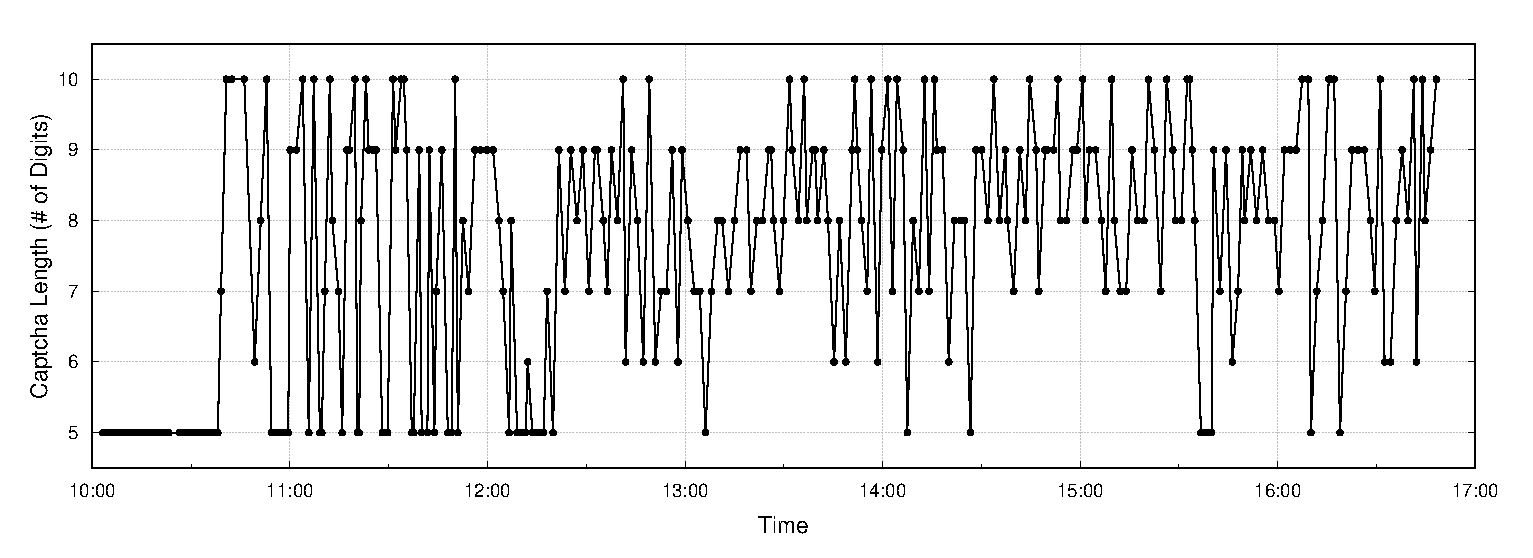
\includegraphics[width=1\textwidth]{figures/captcha_length.eps}
    \label{fig:length_time}
\end{subfigure} %\hspace{0.03\textwidth}
\begin{subfigure}{0.2\textwidth}
    \centering
    %\caption{Average solution time for each recognition service and accent against the audio captcha services we evaluated.}
    \label{tab:length}
    \begin{tabular}{lc}
    \toprule
    \textbf{Digits} & \textbf{\# of Captchas} \\
    \hline
    5 & 95 (31.3\%) \\
    \rowcolor{Gray} 
    6 & 14 (4.6\%) \\
    7 & 34 (11.2\%) \\
    \rowcolor{Gray} 
    8 & 51 (16.8\%) \\
    9 & 68 (22.4\%) \\
    \rowcolor{Gray} 
    10 & 41 (13.5\%)\\
    \bottomrule
    \end{tabular}
\end{subfigure}
\caption{Variation of audio captcha length in \re v2.0 over time.}
\label{fig:length}
\end{figure*}

\textbf{\re.} While our study aims to evaluate the robustness of many popular audio captchas, 
Google's \re is the most prevalent captcha service, so we offer some interesting details 
and findings from our experiments.

\emph{Bypassing rate limits.} As aforementioned in Section~\ref{sec:recaptcha}, \re enforces 
rate limiting to prevent large scale attacks from a small number of machines. While in practice
captcha solving services employ proxies~\cite{captcha_proxies} and botnets (e.g., KoobFace~\cite{captcha_solvers}) 
to overcome such limits, we further explored this mechanism during our experiments. Initially,
we employed a straightforward approach of circulating through a list of valid User Agent strings,
so as to masquerade as numerous computers connecting from a single IP address (e.g., users behind a NAT).
However, in that case \re would enforce the same limit. Surprisingly, though, we found that if we 
supplied a bogus nonsensical User Agent we were able to completely bypass the rate limiting,
and only faced issues when issuing many concurrent solvers (which could be flagged as a potential DDoS attempt).
%solving  well over a thousand captchas per day from a single IP address. 
We surmise that a bug in the risk analysis
system does not enforce the check on the other aspects of the request (e.g., IP address, HTTP cookies) when
it encounters an ``invalid'' User Agent\footnote{This issue has now been fixed.}.
%This incident 
%further highlights how seemingly complex captcha services ]

\emph{Adaptive length}.
While by default the length of \re v2.0 was 5 digits, we found %that after multiple captcha solutions by our system,
that \re would adapt when facing a large amount of requests from our system and return captchas with more digits. 
In Figure~\ref{fig:length} we present a representative experiment that depicts the number of digits in the captchas
processed by our system over the course of 7 hours. The first 49 captchas all contained 5 digits, whereas the length
changed in a seemingly random fashion. As can be seen by the breakdown statistics in the Figure, apart from the default
version with 5 digits, the most common variation we came across contained 9 digits.
%Overall, out of the 303 challenged processed in the experiment, 95 (31.3\%)
%had a length of 5, 14 (4.6\%) had 6 digits, 34 (11.2\%) had 7, 51 (16.8\%) had 8 digits, 68 (22.4\%) had 9, and 41 
%(13.5\%) had 10 digits.

\begin{figure*}[tp]
\begin{subfigure}{0.24\textwidth}
\includegraphics[width=\textwidth]{figures/recaptcha_evolution/2011.pdf}
\caption{\re cca. 2011}
\label{fig:apple}
\end{subfigure} \hspace{0.01\textwidth}
\begin{subfigure}{0.24\textwidth}
\includegraphics[width=\textwidth]{figures/recaptcha_evolution/2014b.pdf}
\caption{\re cca. 2014}
\label{fig:botdetect}
\end{subfigure}\hspace{0.01\textwidth}
\begin{subfigure}{0.24\textwidth}
\includegraphics[width=\textwidth]{figures/recaptcha_evolution/2016.pdf}
\caption{\re cca. 2015-2016}
\label{fig:captchas}
\end{subfigure}
\begin{subfigure}{0.24\textwidth}
\includegraphics[width=\textwidth]{figures/recaptcha_evolution/2017.pdf}
\caption{\re after March 2017}
\label{fig:live}
\end{subfigure}
\caption{The evolution of \re audio challenges through time.}
\label{fig:evolution}
\end{figure*}


\emph{Evolution through time.} In their extensive user study on the usability of captchas, Burzstein et al.~\cite{captchas-are-hard}
found that users were able to solve only 47\% of \re's audio challenges (that number was calculated following an optimistic approach
and is an upper bound to the actual accuracy). Since then \re has modified their audio challenges. % to be more user friendly.
Here we further explore how audio \re has evolved through time. 

In Figure~\ref{fig:evolution} we visualize audio captcha samples
that capture \re's evolution through time. Indeed, the audio challenges from 2011 are the least ``user-friendly'' as they contain
a significant amount of background noise in the form of unintelligible discussions, reversed recordings of speech. While the version
from 2014 is considerably clearer and only five digits long, the audio quality of the spoken digits remains ``noisy'', while background recordings were
also sporadically interjected. In the sample plotted here, a background recording uttering ``three'' is almost overlapping with the
digit spoken as part of the challenge (shown in red). As part of their ``No Captcha Recaptcha'' system released in December 2014, the audio challenges were 
more simplified as they contained five digits with less noise in the recordings; however, certain recordings are processed and the sounds
are more drawn out. This could potentially be a countermeasure against automated attacks. 
Finally, in the current version which was released in March 2017,
the challenges once again contain 10 digits. 

While there might have been more intermediary changes apart from the ones presented here,
this samples show a clear evolution of audio \re challenges towards a more user-friendly scheme. The change in the latest version 
is most likely an attempt to mitigate automated attacks; however, this can only serve as a temporary measure as our experiments
demonstrate that speech recognition technology has reached a point where such challenges can be trivially bypassed. Thus, it remains 
to be seen whether \re adopts an approach similar to services like Securimage and BotDetect and reverts back to challenges with 
more noise and distortion to hinder automated attacks.

\section{Discussion}
\label{sec:discussion}

How can we fix this problem? The amount of noise we can add before an audio captcha becomes unusable is 
far more constrained than for visual challenges.

Human hearing is more error prone than vision~\cite{o2009auditory,shinn2008object}.

\section{Deep Learning}
\label{sec:deeplearning}

Deep Learning is relatively new area in Machine learning that uses many layers of processing units to extract feature information and create a classification model. It is intended to make a system more artificially intelligent by training on huge datasets. We looked at this class of machine learning for creating an offline solver for Audio CAPTCHAs. Since we had very low rates of accuracy for Securimage and Live, we looked to create separate classification models for them.\newline

To do this, we used Intel NervanaSystem's open-source deep learning library for speech recognition called \textbf{deepspeech}. The source code for this library can be accessed from their GitHub URL (https://github.com/NervanaSystems\newline deepspeech). Their implementation is based on Baidu SVAIL's Deep Speech 2 in neon [].\newline

We installed deepspeech on a machine with 16GB RAM and an NVIDIA Titan X GPU card. We are in the process of training the system with a dataset of 10,000 CAPTCHA files from Securimage along with their truth values. Once trained, the model can be used to predict transcriptions for audio CAPTCHAs obtained at real-time. 

\section{Future Work}
\label{sec:future}

As mentioned earlier, we are looking to create our own classifiers with an off-the-shelf open-source deep learning library for speech recognition. We intend to do this for each CAPTCHA system by training with datasets collected from all our previous experimental runs and evaluations. Our focus is mainly towards Securimage and Microsoft Live since we have low accuracy rates for both of them.\newline

We also intend to look into 2 other CAPTCHA systems - Mollom and SolveMedia both of which are being used by some popular websites.\newline
\section{Conclusions}
\label{sec:conclusions}

What did we do?

\section{References}


1. Tam, Jennifer, et al. "Breaking Audio CAPTCHAs." NIPS. 2008. \newline
2. Tam, Jennifer, et al. "Improving audio captchas." Symposium On Usable Privacy and Security (SOUPS). 2008.\newline
3. Aiswarya, K., and K. S. Kuppusamy. "A Study of Audio Captcha and their Limitations."\newline
4. Breaking Google's audio CAPTCHA: http://www.\newline
networkworld.com/article/2278947/lan-wan/breaking-google-s-audio-captcha.html\newline
5. Bursztein, Elie, and Steven Bethard. "Decaptcha: breaking 75\% of eBay audio CAPTCHAs." Proceedings of the 3rd USENIX conference on Offensive technologies. USENIX Association, 2009.\newline
6. Meutzner, Hendrik, et al. "Using automatic speech recognition for attacking acoustic CAPTCHAs: The trade-off between usability and security." Proceedings of the 30th Annual Computer Security Applications Conference. ACM, 2014.\newline
7. Darnstädt, Malte, Hendrik Meutzner, and Dorothea Kolossa. "Reducing the Cost of Breaking Audio CAPTCHAs by Active and Semi-supervised Learning." Machine Learning and Applications (ICMLA), 2014 13th International Conference on. IEEE, 2014.\newline
8. Bursztein, Elie, et al. "The failure of noise-based non-continuous audio captchas." Security and Privacy (SP), 2011 IEEE Symposium on. IEEE, 2011.\newline
9. Sivakorn, Suphannee, Iasonas Polakis, and Angelos D. Keromytis. "The cracked cookie jar: HTTP cookie hijacking and the exposure of private information." Security and Privacy (SP), 2016 IEEE Symposium on. IEEE, 2016.\newline
10. Amodei, Dario, et al. "Deep speech 2: End-to-end speech recognition in english and mandarin." arXiv preprint arXiv:1512.02595 (2015).


\end{document}


